\documentclass{book}
\renewcommand{\familydefault}{\sfdefault}

%\usepackage{libertine}
\usepackage{amsmath}
\usepackage{graphicx}	
\usepackage{amssymb}
\usepackage{epstopdf}
\usepackage{adjustbox}
\usepackage{array}
\usepackage{color}
\usepackage{pdflscape}
\usepackage{minted}
\usepackage{colortbl}
\usepackage{subcaption}

\usepackage{algorithm}
\usepackage{algorithmic}

\usepackage{tikz}

\usepackage[top=3cm,bottom=3cm,left=3cm,right=3cm,headsep=10pt,a4paper]{geometry} % Page margins

\usepackage{graphicx} 
\usepackage{titlepic}
%\usepackage{pstricks}

\usepackage[calcwidth]{titlesec}
\newlength\mylen
%\setlength\mylen{\dimexpr\oddsidemargin+1in+\hoffset\relax}
\setlength\mylen{\dimexpr\oddsidemargin+20pt+\hoffset\relax}
\titleformat{\section}
  {\normalfont\Large\bfseries}
  {\llap{\hspace*{-\mylen}\thesection\hfill}}{0em}{}
  [{\makebox[\linewidth][l]{%
    \hspace*{-\mylen}\rule{\dimexpr\textwidth+\mylen\relax}{1pt}}}]


\usepackage[framemethod=TikZ]{mdframed}
\mdfdefinestyle{MyFrame}{%
    linecolor=blue,
    outerlinewidth=2pt,
    roundcorner=20pt,
    innertopmargin=\baselineskip,
    innerbottommargin=\baselineskip,
    innerrightmargin=20pt,
    innerleftmargin=20pt,
    backgroundcolor=gray!50!white}

\mdfdefinestyle{cli}{%
    linecolor=none,
    outerlinewidth=2pt,
    roundcorner=5pt,
    innertopmargin=\baselineskip,
    innerbottommargin=\baselineskip,
    innerrightmargin=10pt,
    innerleftmargin=10pt,
    backgroundcolor=gray!10!white}


\mdfdefinestyle{aaa}{%
  topline=false,rightline=false,bottomline=false,
  frametitlerule=true,innertopmargin=10pt,
  outerlinewidth=3pt,outerlinecolor=gray,
  pstricksappsetting={\addtopsstyle{mdfouterlinestyle}{linestyle=dashed}},innerlinecolor=black,innerlinewidth=0pt}
 
%\usepackage{tikz}
%\usetikzlibrary{arrows,automata}

\usepackage{hyperref}
\hypersetup{
    colorlinks = true,
    linkcolor = {blue},
    linkbordercolor = {gray},
    citecolor = {blue}
}

\DeclareGraphicsRule{.tif}{png}{.png}{`convert #1 `dirname #1`/`basename #1 .tif`.png}

\newcommand{\CP}[2]{\text{{\bf P[}$ #1 \mid #2 ${\bf ]}}}
\newcommand{\PR}[1]{\text{{\bf P[}$#1${\bf]}}}
\newcommand{\F}{{\cal F}}
\newcommand{\M}{{\textsc{M}}}
\newcommand{\A}{{\textsc{A}}}



%\titlepic{\includegraphics[width=\textwidth]{joy-album.png}}
%\title{\huge Using \text{Joy}} 
%\author{David McGrew and others\\ \texttt{\{mcgrew\}@cisco.com} } 
%\institute{Cisco Systems, Inc. } 
%\date{\today}

%\definecolor{titlepagecolor}{cmyk}{1,.60,0,.40}
%\definecolor{titlepagecolor}{cmyk}{.16,.12,.13,.0}
\definecolor{titlepagecolor}{cmyk}{0,0,0,.3}
\definecolor{namecolor}{cmyk}{1,.50,0,.10} 
\definecolor{darkgray}{cmyk}{0,0,0,.27} 
\begin{document}
%\pagecolor{titlepagecolor}
%\maketitle

\begin{titlepage}
\newgeometry{left=3cm} 
%\newgeometry{left=5cm} 
\pagecolor{titlepagecolor}
\noindent

\includegraphics[width=2.5in]{joy-icon.png}\\[-1em]
\color{white}
\rule{1\textwidth}{1pt} \\ \vspace{11pt}
\par
\noindent
\textbf{ \huge {\textsf{A package for capturing and analyzing network data features}}}
\vfill
\noindent
%{\huge \textsf{David McGrew, etc.}}
\vskip\baselineskip
\noindent
\textsf{ \huge \hfill Joy version 2.0}

\textsf{ \huge \hfill January 2018}
\end{titlepage}
\restoregeometry % restores the geometry
\pagecolor{white}

\frontmatter
\chapter{Preface}
\text{Joy} is a BSD-licensed open source software package for
collecting and analyzing network data, with a focus on network data
feature exploration.  This document shows how it can be used,
installed, built, and modified.  We hope that you find it useful, and
that you enjoy using it.  Please do understand that it is open source
software, with the following licensing terms:

\begin{quote}
Copyright \copyright \, 2018 Cisco Systems \\
All rights reserved. \\
 
Redistribution and use in source and binary forms, with or without
modification, are permitted provided that the following conditions are
met:
\begin{enumerate}
  \item Redistributions of source code must retain the above copyright
    notice, this list of conditions and the following disclaimer.
 
  \item Redistributions in binary form must reproduce the above
   copyright notice, this list of conditions and the following
   disclaimer in the documentation and/or other materials provided
   with the distribution.
 
   \item Neither the name of the Cisco Systems, Inc. nor the names of its
   contributors may be used to endorse or promote products derived
   from this software without specific prior written permission.
\end{enumerate}
   
 THIS SOFTWARE IS PROVIDED BY THE COPYRIGHT HOLDERS AND CONTRIBUTORS
 "AS IS" AND ANY EXPRESS OR IMPLIED WARRANTIES, INCLUDING, BUT NOT
 LIMITED TO, THE IMPLIED WARRANTIES OF MERCHANTABILITY AND FITNESS
 FOR A PARTICULAR PURPOSE ARE DISCLAIMED. IN NO EVENT SHALL THE
 COPYRIGHT HOLDERS OR CONTRIBUTORS BE LIABLE FOR ANY DIRECT,
 INDIRECT, INCIDENTAL, SPECIAL, EXEMPLARY, OR CONSEQUENTIAL DAMAGES
 (INCLUDING, BUT NOT LIMITED TO, PROCUREMENT OF SUBSTITUTE GOODS OR
 SERVICES; LOSS OF USE, DATA, OR PROFITS; OR BUSINESS INTERRUPTION)
 HOWEVER CAUSED AND ON ANY THEORY OF LIABILITY, WHETHER IN CONTRACT,
 STRICT LIABILITY, OR TORT (INCLUDING NEGLIGENCE OR OTHERWISE)
 ARISING IN ANY WAY OUT OF THE USE OF THIS SOFTWARE, EVEN IF ADVISED
 OF THE POSSIBILITY OF SUCH DAMAGE.

\end{quote}

We gratefully acknowledge the support of our employer for the
development of this package, and to the people who contributed to it,
including Ellie Daw and Luke Valenta.

\begin{quote}
\textit{ -- the Joy team: Philip Perricone, Bill Hudson, Blake Anderson, Brian Long, and David McGrew}
\end{quote}




\mainmatter

\tableofcontents





\chapter{Introduction}

\section{Overview}
The \text{Joy} package contains a data collection program,
\texttt{joy}, and some data analysis programs, including
\texttt{sleuth}.  The former is written in C99, and it reads raw
network traffic or a packet capture file, and then outputs a summary
of the observed traffic in JavaScript Object Notation
(JSON)~\cite{rfc7159} format; see Figure~\ref{example} for an example.
That program can also operate in telemetry collector mode, and receive
IPFIX
or Netflow version~9 packets; in that mode, it translates
the telemetry into a JSON description of the flows that are observed
by the telemetry exporters.  The \texttt{sleuth} program reads a JSON
description of traffic, filters the traffic as specified on its
command line, and prints out the description of selected traffic, or
it can select, summarize, or analyze traffic, as described in
Section~\ref{querytool}.

\begin{figure}
  \caption{An example JSON description of a unidirectional flow.  See
    Figure~\ref{examplefig} for an illustration of this flow.  }
  \label{example}.
\begin{minted}{javascript}
{
  "sa": "0.0.0.0",                    // IP source address
  "da": "255.255.255.255",            // IP destination address
  "pr": 17,                           // IP protocol number (17 = UDP)
  "sp": 68,                           // UDP source port 
  "dp": 67,                           // UDP destination port
  "bytes_out": 900,                   // bytes sent from sa to da
  "num_pkts_out": 3,                  // packets sent from sa to da
  "time_start": 1479227824.653818,    // start time in seconds since the epoch
  "time_end": 1479227829.665744,      // end time in seconds since the epoch
  "packets": [                        // array of packet information
    {                                  
      "b": 300,                       // bytes in UDP Data field
      "dir": ">",                     // direction: sa -> da
      "ipt": 0                        // inter-packet time: 0 ms since time_start
    },
    {
      "b": 300,                       // bytes in UDP Data field
      "dir": ">",                     // direction: sa -> da
      "ipt": 5006                     // inter-packet time: 5006 ms since last packet
    },
    {
      "b": 300,                       // bytes in UDP Data field
      "dir": ">",                     // direction: sa -> da
      "ipt": 4                        // inter-packet time: 4 ms since last packet
    }
  ],
  "ip": {                            
    "out": {
      "ttl": 128,
      "id": [
        1,
        2,
        3
      ]
    }
  },
  "expire_type": "i"
}
\end{minted}
\end{figure}


\begin{figure}
  \caption{An illustration of the example unidirectional flow from
    Figure~\ref{example}, showing the relationship between the
    \texttt{start\_time}, \texttt{stop\_time}, and the \texttt{ipt}
    (inter-packet time) values.  The first \texttt{ipt} value is
    zero.}
\label{examplefig}
\begin{center}
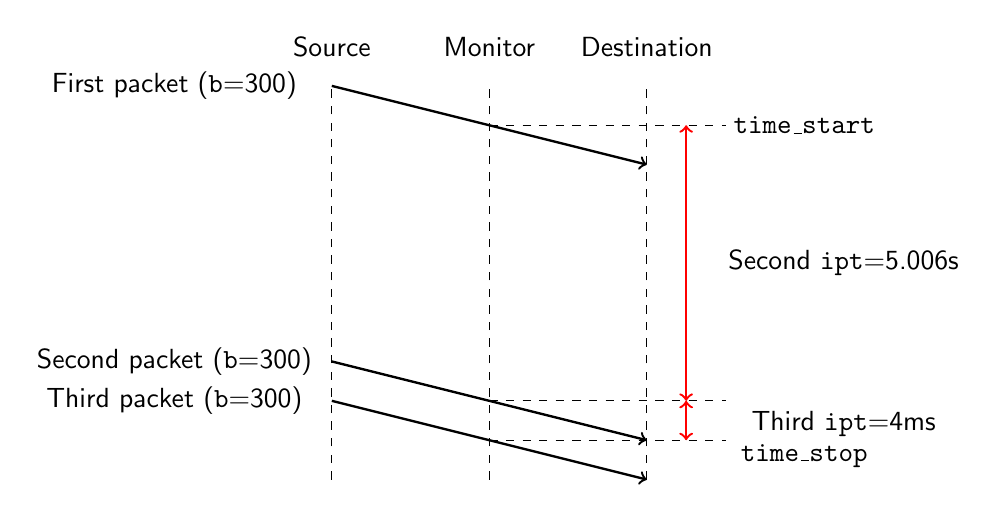
\begin{tikzpicture}
\node at (4,7.5) {Destination};
\node at (2,7.5) {Monitor};
\node at (0,7.5) {Source};
\draw[dashed] (0,2) -- (0,7);  
\draw[dashed] (4,2) -- (4,7);
\draw[dashed] (2,2) -- (2,7);  
\node at (-2,7) {First packet (\texttt{b}=300)};
\draw[line width=.3mm,->] (0,7) -- (4,6);
%\node at (-2,5.5) {TCP SYN/ACK (\texttt{b}=0)};
%\draw[line width=.3mm,->] (4,6) -- (0,5);
\draw[dashed] (2,6.5) -- (5,6.5);
\node at (4.5,6) {};
\node at (6,6.5) {\texttt{time\_start}};
%\draw[dashed] (2,5.5) -- (5,5.5);
\node at (-2,3.5) {Second packet (\texttt{b}=300)};
\node at (6,5.5) {};
\draw[line width=.3mm,<->,red] (4.5,6.5) -- (4.5,3);
\node at (6.5,4.75) {Second \texttt{ipt}=5.006s};
\draw[line width=.3mm,->] (0,3.5) -- (4,2.5);
\draw[line width=.3mm,->] (0,3) -- (4,2);
\draw[dashed] (2,3) -- (5,3);
\node at (6,4.5) {};
\draw[dashed] (2,2.5) -- (5,2.5);
\node at (6,2.3) {\texttt{time\_stop}};
\node at (-2,3) {Third packet (\texttt{b}=300)};
\node at (6,2.5) {};
\draw[line width=.3mm,<->,red] (4.5,3) -- (4.5,2.5);
%\draw[line width=.3mm,<->,blue] (4,4) -- (4,3);
\node at (6.5,2.7) {Third \texttt{ipt}=4ms};
\node at (4.5,3.5) {};
\end{tikzpicture}
\end{center}
\end{figure}


\subsection{Why \text{Joy}?}
\text{Joy} is useful for collecting, analyzing, and exploring
network data.  Its JSON output formats are flexible and well-suited
for many data analysis tools and modern programming environments, such
as \texttt{python} and \texttt{scikit-learn}, and it uses a
flow-oriented model that is both convenient and conceptually familiar.
It can obtain network metadata while preserving privacy, by avoiding
bulk data capture and by anonymizing addresses and usernames.  It is
aware of several important protocols, including HTTP, TLS, DNS, and
DHCP, in the sense of being able to record their session metadata
elements in its JSON format.  It is also easily extensible; JSON
gracefully handles optional or additional data, and the capture tool
has a C preprocessor interface facilitating the capture of new data
elements.

\text{Joy} does not know about as many protocols as do
\texttt{wireshark}, \texttt{tshark}, or \texttt{tcpdump}, so the
latter tools may be better suited for a detailed human-driven forensic
analysis of a particular packet capture file.  However, \text{Joy}
is better suited for analyzing many sessions or many packet capture
files.

%\text{Joy} captures data for each flow, unlike traditional Intrusion
%Detection Systems (IDS) or Intrusion Protection Systems (IPS) like
%Snort or Bro, which generate alerts for security-relevant events that
%they detect.  The less verbose nature of IDS systems is better suited
%for high-bandwidth scenarios.  \text{Joy} also does not implement a
%session-blocking facility, as would a complete IPS.

Flow, in positive psychology, is a state in which a person
performing an activity is fully immersed in a feeling of energized
focus, deep involvement, and joy.  This second meaning inspired
the choice of name for this software package.

\subsection{Ethics}
Joy is intended for use in network and security research, forensics,
and for the monitoring of (small scale) networks to detect
vulnerabilities, threats and other unauthorized or unwanted behavior.
Researchers, administrators, penetration testers, and security
operations teams can put this information to good use, for the
protection of the networks being monitored, and in the case of
vulnerabilities, for the benefit of the broader community through
improved defensive posture.  As with any network monitoring tool, Joy
could potentially be misused; \textbf{do not use it on any network of
  which you are not the owner or the administrator}.

% Goofus flagrantly violates the privacy of others by running joy in
% promiscuous mode without their awareness and consent. 
%
% Gallant always anonymizes addresses and usernames, even when the
% network owner authorizes him to run joy off of a network tap.


%\subsection{Trivia}


\section{Network data background}
A \textit{flow} is a set of packets with common characteristics,
called a \textit{flow key}. In \text{Joy}, the flow key is the
conventional network five-tuple: the source and destination addresses,
the source and destination port (for TCP and UDP traffic) and the
protocol number.  Symbolically, a flow key is the tuple (\texttt{sa,
  da, pr, sp, dp}).  As defined above, a flow is
\textit{unidirectional}; all of its packets move in the same
direction.  Interactive network sessions usually involve
\textit{bidirectional} flows, which are described in Section~\ref{biflow}.

In this document, we sometimes use the term flow
to mean a data record that describes a flow; this convention is
commonplace in computer networking.
%Netflow version~5
%has a fixed set of basic data elements;
The following table shows the flow key fields in the JSON format that \text{Joy} uses,
along with some other important ones:\\
\begin{center}
\begin{tabular}{l|l|l}
JSON element             & Data element                           & Notes            \\ \hline
\texttt{sa}              & Source Address                         & Internet Protocol   \\
\texttt{da}              & Destination Address                    &                     \\
\texttt{pr}              & Protocol Number                        &                     \\ \hline
\texttt{sp}              & Source Port                            & TCP or UDP          \\
\texttt{dp}              & Destination Port                       &                     \\ \hline
\texttt{bytes\_out}      & Number of bytes sa$\rightarrow$da      & Any Protocol        \\ 
                         & in TCP, UDP, ICMP, or IP Data fields   &                    \\ 
\texttt{num\_pkts\_out}  & Number of packets sa$\rightarrow$da    &                     \\ 
\texttt{time\_start}     & Start time, seconds since epoch        &                     \\
\texttt{time\_end}       & End time, seconds since epoch          &                     \\ 
\texttt{packets}         & Array of packet lengths, directions, and times &                \\ \hline \rowcolor{lightgray}
\texttt{bytes\_in}      & Number of bytes sa$\leftarrow$da       & Bidirectional flows only  \\ \rowcolor{lightgray}
                         & in TCP, UDP, ICMP, or IP Data fields   &                    \\ \rowcolor{lightgray}
\texttt{num\_pkts\_in}  & Number of packets sa$\leftarrow$da      &                    
\end{tabular}\\
\end{center}
The epoch is defined by POSIX as 00:00:00 Coordinated Universal Time
(UTC), Thursday, 1 January 1970.

By default, \texttt{joy} does \textbf{not} report TCP packets with a
zero-length Data field in the \texttt{packets} array.  All TCP
sessions start out with a handshake that contains two such packets,
and most TCP sessions include 'ACK packets' that contain no data, and
serve only to acknowledge the receipt of data sent by the other side.
See Section~\ref{zeros} for more information.

\text{Joy} extracts protocol-specific metadata, such as HTTP headers,
TLS certificates, or DNS request names, and stores the data for each
protocol in a JSON sub-object, such as \texttt{http}, \texttt{tls},
\texttt{dns}.  To capture data for a particular protocol, the
appropriate command line option must be passed to \texttt{joy}, as
described in Section~\ref{dataopts}.  To select particular data
elements from each flow, the \texttt{sleuth --select} facility can be
used, as described in Section~\ref{selectopt}.


\subsection{Bidirectional flows}
\label{biflow}
By default, \texttt{joy} captures unidirectional flows, but in many
cases, bidirectional flows are more interesting; the \texttt{bidir=1}
option (Section~\ref{bidir}) causes that program to stitch together
any unidirectional flows that are part of the same session.  A
\textit{bidirectional} flow consists of a pair of unidirectional flows
whose source and destination addresses and ports are reversed, and
whose time spans overlap.  That is, if the flows \texttt{out} and
\texttt{in} are unidirectional, then their combination is a
bidirectional flow when
\begin{align}                          \nonumber
\texttt{in.sa} & = \texttt{out.da}, \\ \nonumber
\texttt{in.da} & = \texttt{out.sa}, \\ \nonumber
\texttt{in.sp} & = \texttt{out.dp}, \\ 
\texttt{in.dp} & = \texttt{out.sp}, \\ \nonumber
\texttt{in.pr} & = \texttt{out.pr}, \\ \nonumber
\texttt{in.start\_time} & > \texttt{out.start\_time}, \\ \nonumber
\texttt{in.start\_time} & < \texttt{out.stop\_time}. \\ \nonumber
\end{align}
Figure~\ref{biflowexample} shows the relationship between two
unidirectional flows and their bidirectional combination, and
Figure~\ref{biexample} shows an example Joy output for a bidirectional
flow.  Joy uses the convention that, in a bidirectional flow, the
packets flowing from \texttt{sa} (source) to \texttt{da} (destination)
are \textit{outbound}, and the packets flowing from \texttt{da} to
\texttt{sa} are \textit{inbound}; whenever \texttt{out} and
\texttt{in} are used in the JSON schema, this directionality is
implied.

A bidirectional flow is sometimes called a \textit{biflow}.

\begin{figure}
  \centering
\caption{Bidirectional flow examples.}
\begin{subfigure}{.45\textwidth}
  \centering
  \caption{ The correspondence between a bidirectional flow and its
    component outbound (black) and inbound (grey) unidirectional
    flows. }
\label{biflowexample}
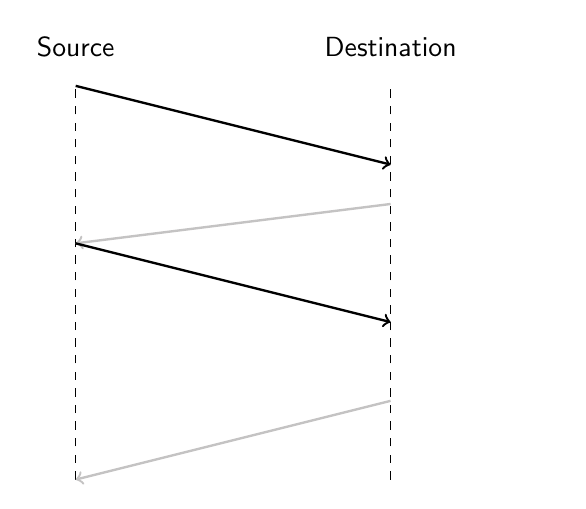
\begin{tikzpicture}
\node at (4,7.5) {Destination};
%\node at (2,7.5) {Monitor};
\node at (0,7.5) {Source};
\draw[dashed] (0,2) -- (0,7);  
\draw[dashed] (4,2) -- (4,7);
%\draw[dashed] (2,2) -- (2,7);  
%\node at (-2,6.5) {TCP SYN (\texttt{b}=0)};
\draw[line width=.3mm,->] (0,7) -- (4,6);
%\node at (-2,5.5) {TCP SYN/ACK (\texttt{b}=0)};
\draw[line width=.3mm,->,darkgray] (4,5.5) -- (0,5);
%\draw[dashed] (2,6.5) -- (5,6.5);
\node at (4.5,6) {};
%\node at (6,6.5) {\texttt{time\_start}};
%\draw[dashed] (2,5.5) -- (5,5.5);
%\node at (-2,4.5) {TCP Data ($\texttt{b}>0$)};
\node at (6,5.5) {};
%\draw[line width=.3mm,<->,red] (4.5,6.5) -- (4.5,4.5);
%\node at (5.5,5.5) {First \texttt{ipt}};
\draw[line width=.3mm,->] (0,5) -- (4,4);
\draw[line width=.3mm,->,darkgray] (4,3) -- (0,2);
%\draw[dashed] (2,4.5) -- (5,4.5);
\node at (6,4.5) {};
%\draw[dashed] (2,2.5) -- (5,2.5);
%\node at (-2,2.5) {TCP Data ($\texttt{b}>0$)};
\node at (6,2.5) {};
%\draw[line width=.3mm,<->,red] (4.5,4.5) -- (4.5,2.5);
%\draw[line width=.3mm,<->,blue] (4,4) -- (4,3);
%\node at (5.5,3.5) {Second \texttt{ipt}};
\node at (4.5,3.5) {};
\end{tikzpicture}
\end{subfigure}
\hspace{22pt}
\begin{subfigure}{.45\textwidth}
  \centering
  \subcaption{A JSON example of a bidirectional flow,
  noting inbound data elements.}
  \label{biexample}
\begin{minted}{javascript}
{
  "sa": "172.16.87.100",
  "da": "52.72.161.26",
  "pr": 6,
  "sp": 49173,
  "dp": 443,
  "bytes_out": 338,
  "num_pkts_out": 7,
  "bytes_in": 5629,     // inbound                
  "num_pkts_in": 9,     // inbound                
  "time_start": 1479227853.446511,
  "time_end": 1479227854.969042,
  ...
}
\end{minted}
\end{subfigure}
\end{figure}

\subsection{Flow expiration}
\label{expiration}
It is undesirable, in network monitoring, to wait for a long duration
flow to finish before its flow record becomes available.  Some flows
last nearly as long as the uptime of the operating systems to which
they connect.  To avoid this indefinite wait for flow data, monitoring
systems use a \textit{timeout} approach: a flow record is exported
whenever a flow is inactive for an \textit{inactive timeout} period,
or whenever it is active and its duration exceeds an \textit{active
  timeout} period.  The \texttt{joy} capture tool uses these
conventions, with an inactive timeout period of ten seconds, and an
active timeout period of thirty seconds.  That is, a flow record will
be created if a flow is inactive for ten seconds, or if it is active
for thirty seconds.  The flow record indicates which of these
conditions happened, in the \texttt{expire\_type} element, which
appears in the top level of each flow object:
\begin{itemize}
  \item \texttt{"expire\_type": "i"} denotes an inactive expiration, and
  \item \texttt{"expire\_type": "a"} denotes an active expiration.
\end{itemize}
The \texttt{sleuth} program by default stitches together successive
flows that have matching flow keys.  Chronological stitching can be
turned off (see Section~\ref{nostitch}), which can be useful to
understand how the timeout logic of Netflow or IPFIX monitoring
systems affects data capture.  However, in most cases, chronological
stitching should be used.  This is especially true when monitoring a
private network, because flows that undergo active timeouts
\textbf{can appear to originate outside the private network}.  More to
the point: a lack of chronological stitching can make it appear that
there are flows that violate a private network access control policy.
The TCP SYN flag can be used as a sanity check, since a long-running
TCP flow that is truncated into two more flow records by an active
timeout will only contain a SYN flag in the first flow record.




\chapter{The \texttt{joy} tool}
\label{joytool}
The command line syntax to invoke joy is
\begin{mdframed}[style=aaa]
  \begin{minted}{bash}
joy [options] [file1 [file2 ... ]]
  \end{minted}
\end{mdframed}
By default, its output is GZIP compressed JSON, using the format
described in Section~\ref{chapterschema}.  Uncompressed output, or
\texttt{bz2} compressed output, are available as compile-time options
(see the file \texttt{src/include/output.h}).  There are many software
tools that work with GZIP compressed data, especially on Linux and
other POSIX environments, such as \texttt{gunzip}, \texttt{zless}, and
\texttt{zcat}.   An example invocation that applies \texttt{joy} in offline mode and
uses \texttt{gunzip} to convert its output to uncompressed form:
\begin{mdframed}[style=cli]
\begin{minted}{bash}
joy bidir=1 browse.pcap | gunzip 
\end{minted}
\begin{minted}{javascript}
{"version":"1.74","interface":"none","promisc":0,"output":"none", ... }
{"sa":"10.0.2.15","da":"74.125.228.207","pr":6,"sp":43039,"dp":443, ... }
{"sa":"10.0.2.15","da":"74.125.228.195","pr":6,"sp":54210,"dp":443, ... }
{"sa":"10.0.2.15","da":"74.125.228.104","pr":6,"sp":47443,"dp":443, ... }
...
\end{minted}
\end{mdframed}

\section{Overview}
Each \texttt{joy} option (except \texttt{-x}) has the form \texttt{option=value},
where \texttt{option} is a string that identifies the option, and
\texttt{value} is either a boolean (\texttt{0} or \texttt{1}), a
(nonnegative) number, or a character string.  There are two types of options:
general ones (\ref{generalopts}) and ones that control data features
that are output (\ref{dataopts}).

Joy can be run in several different modes.   In \textbf{offline mode},
joy processes one or more packet capture (PCAP) files and prints
a (compressed) JSON summary of the network flows to \texttt{stdout};
this mode is indicated by one or more file names on the command line.
The file names \textit{must} follow any options that are present,
and each file name \textit{should not} contain the equals sign
(\texttt{=}), to avoid the possibility that joy would
confuse a PCAP file with an option.  

In \textbf{online mode}, joy listens to one or more network
interfaces.  This mode is indicated by using the \texttt{interface=I}
option (Section~\ref{interface}) to specify the interface \texttt{I}.
If the option \texttt{output=F} (Section~\ref{output}) is present,
then the (compressed) JSON output is written to file \texttt{F}.  In
this mode, output file rotation can be specified with \texttt{count}
(Section~\ref{count}), and a log file can be specified with
\texttt{logfile} (Section~\ref{logfile}).  Output files can be
uploaded to a separate server via SCP with the \texttt{upload} option
(Section~\ref{upload}).  Online mode requires \texttt{root} privileges
on most operating systems; for security, \texttt{joy} will drop its
privileges after starting a capture (Section~\ref{username}).

Joy can also be used in Netflow or IPFIX \textbf{collector mode}
(Sections~\ref{ipfixcollectport}, \ref{ipfixcollectonline}) or IPFIX
\textbf{exporter mode} (Sections~\ref{ipfixexportport},
\ref{ipfixexportremoteport}, and \ref{ipfixexportremotehost}).

\subsection{Configuration object}
At initialization and before any other output, \texttt{joy} writes out
a JSON object that describes its complete configuration, and the
version of the \texttt{joy} program that produced it.  This
information is important, because the options affect what data
elements can appear in the flow objects.  Programs that analyze the
\texttt{joy} JSON output \textit{should} check for the configuration
object and make sure that they do not process it as though it were a
flow object, and they \textit{should} do this by checking
for the presence of the \texttt{version} field at the top level
of the object.  An annotated example of a configuration object:
\begin{mdframed}[style=cli]
\begin{minted}{javascript}
{
  "version":"1.74",      // version of joy program 
  "interface":"none",    // no output interface specified
  "promisc":0,           // no promiscuous mode
  "output":"none",       // no output specified; stdout will be used
  "outputdir":"none",    // no output directory specified
  "username":"none",     // no username specified for privilege dropping
  ...
}
\end{minted}
\end{mdframed}
The JSON names in the configuration object are \texttt{joy} command
names, as defined in this chapter.  


\subsection{Subnet files}
\label{subnet}
Some options cause \texttt{joy} to read a set of subnets from a file,
and perform specific processing when \texttt{sa} and/or \texttt{da}
are in one of those subnets.  The format of a subnet file is
illustrated by file \texttt{internal.net}:
\begin{mdframed}[style=cli]
\begin{minted}{bash}
# subnets for address anonymization
#

10.0.0.0/8         #  RFC 1918 address space
172.16.0.0/12      #  RFC 1918 address space
192.168.0.0/16     #  RFC 1918 address space
\end{minted}
\end{mdframed}
Each line contains an address as a dotted quad, or a subnet as a
dotted quad followed by a slash and a number between 0 and 32, or is
empty.  A \# character, and any characters on a line following it, are
ignored, as are empty lines.

\section{General options}
\label{generalopts}
%\begin{centering}
%\begin{tabular}{l|l}
%\tt  -x F                                 & read configuration commands from file F \\
%\tt  interface=I                          & read packets live from interface I \\
%\tt  promisc=1                            & put interface into promiscuous mode \\
%\tt  output=F                             & write output to file F (otherwise stdout is used) \\
%\tt  logfile=F                            & write secondary output to file F (otherwise stderr is used) \\
%\tt  count=C                              & rotate output files so each has about C records \\
%\tt  upload=user@server:path              & upload to user@server:path with scp after file rotation \\
%\tt  keyfile=F                            & use SSH identity (private key) in file F for upload \\
%\tt  anon=F                               & anonymize addresses matching the subnets listed in file F \\
%\tt  retain=1                             & retain a local copy of file after upload \\
%\tt  preemptive\_timeout=1                & For active flows, look at incoming packets timestamp to decide if \\
%                                          & adding that packet to the flow record will automatically time it out. \\
%                                          & Default=0 \\
%\tt  nfv9\_port=N                         & enable Netflow V9 capture on port N \\
%\tt  ipfix\_collect\_port=N               & enable IPFIX collector on port N \\
%\tt  ipfix\_collect\_online=1             & use an active UDP socket for IPFIX collector \\
%\tt  ipfix\_export\_port=N                & enable IPFIX export on port N \\
%\tt  ipfix\_export\_remote\_port=N        & IPFIX exporter will send to port N that exists on the remote server target \\
%                                          & Default=4739 \\
%\tt  ipfix\_export\_remote\_host="host"   & Use "host" as the remote server target for the IPFIX exporter \\
%                                          & Default="127.0.0.1" (localhost) \\
%\tt  ipfix\_export\_template="type"       & Use "type" as the template for IPFIX exporter \\
%                                          & Default="simple" (5-tuple) \\
%                                          & Available types: "simple", "idp" \\
%\tt  aux\_resource\_path="path"           & The path to directory where auxillary resources are stored \\
%\tt  verbosity=L                          & Specify the lowest log level \\
%                                          & 0=off, 1=debug, 2=info, 3=warning, 4=error, 5=critical \\
%                                          & Default=4 \\
%\tt  show\_config=0                       & Show the configuration on stderr in the CLI on program run \\
%                                          & 0=off, 1=show \\
%\tt  show\_interfaces=0                   &  Show the interfaces on stderr in the CLI on program run \\
%                                          & 0=off, 1=show \\
%\tt  username="user"                      & Drop privileges to username "user" after starting packet capture \\
%                                          & Default="joy" 
%\end{tabular}
%\end{centering}

\subsection{-x F (string)}
\label{x}
\begin{mdframed}[style=aaa]
Syntax:
  \begin{minted}{bash}
-x F                      
  \end{minted}
\end{mdframed}
The command \texttt{-x F} causes \texttt{joy} to read configuration commands
from the file \texttt{F}.

\subsection{interface=I (string)}
\label{interface}
\begin{mdframed}[style=aaa]
Syntax:
  \begin{minted}{bash}
interface=I               
  \end{minted}
\end{mdframed}
The command \texttt{interface=I} causes \texttt{joy} to read packets
live from network interface \texttt{I}, in online mode.  

\subsection{promisc=1 (boolean)}
\label{promisc}
%The command \texttt{promisc=b} puts the network interface being monitored into promiscuous mode (\texttt{b=1}) or not (\texttt{b=0}).
\begin{mdframed}[style=aaa]
Syntax:
  \begin{minted}{bash}
promisc=1                 
  \end{minted}
\end{mdframed}
If \texttt{promisc=1}, and running in online mode, put the network
interface into promiscuous mode.

\subsection{output=F (string)}
\label{output}
\begin{mdframed}[style=aaa]
Syntax:
  \begin{minted}{bash}
output=F                   
  \end{minted}
\end{mdframed}
Write output to file \texttt{F}; otherwise \texttt{stdout} is used.

\subsection{logfile=F (string)}
\label{logfile}
\begin{mdframed}[style=aaa]
  \begin{minted}{bash}
logfile=F                  
  \end{minted}
\end{mdframed}
Write secondary output to file \texttt{F}; otherwise \texttt{stderr} is used.
Secondary output consists of status reports, warnings, and errors.

\subsection{count=C (number)}
\label{count}
\begin{mdframed}[style=aaa]
Syntax:
  \begin{minted}{bash}
count=C
  \end{minted}
\end{mdframed}
Rotate output files so each contains about \texttt{C} records.  

\subsection{upload=user\@server:path (string)}
\label{upload}
\begin{mdframed}[style=aaa]
  \begin{minted}{bash}
upload=user@server:path    
  \end{minted}
\end{mdframed}
Upload data files using the secure copy utility \texttt{scp}
to the location \texttt{user\@server:path}, after file rotation.

\subsection{keyfile=F (string)}
\label{keyfile}
\begin{mdframed}[style=aaa]
Syntax:
  \begin{minted}{bash}
keyfile=F                  
  \end{minted}
\end{mdframed}
When uploading data files using the \texttt{upload} command (Section~\ref{upload}), use the
SSH identity (private key) in file \texttt{F} to authenticate to the
server.

\subsection{anon=F (string)}
\label{anon}
\begin{mdframed}[style=aaa]
Syntax:
  \begin{minted}{bash}
anon=F                     
  \end{minted}
\end{mdframed}
Anonymize addresses matching the subnets listed in file \texttt{F}.
The format of the subnet file is described in Section~\ref{subnet}.

\subsection{retain=1 (boolean)}
\label{retain}
\begin{mdframed}[style=aaa]
Syntax:
  \begin{minted}{bash}
retain=1                   
  \end{minted}
\end{mdframed}
If \texttt{retain=1}, retain a local copy of each data file after it
is uploaded.  

\subsection{preemptive\_timeout=1 (boolean)}
\label{preemptivetimeout}
\begin{mdframed}[style=aaa]
Syntax:
  \begin{minted}{bash}
preemptive_timeout=1   
  \end{minted}
\end{mdframed}
If \texttt{preemptive\_timeout=1}, then use active flow timeout logic
that uses the packet timestamp to decide if adding that packet to the
flow record would trigger a timeout.

\subsection{nfv9\_port=N (number)}
\label{nfv9port}
\begin{mdframed}[style=aaa]
Syntax:
  \begin{minted}{bash}
nfv9_port=N                
  \end{minted}
\end{mdframed}
If \texttt{nfv9\_port=1}, enable Netflow V9 capture on port \texttt{N}.
Netflow v9~\cite{rfc3954} reports basic flow telemetry.


\subsection{ipfix\_collect\_port=N (number)}
\label{ipfixcollectport}
\begin{mdframed}[style=aaa]
Syntax:
  \begin{minted}{bash}
ipfix_collect_port=N       
  \end{minted}
\end{mdframed}
If \texttt{ipfix\_collect\_port=1}, enable IPFIX capture on port \texttt{N}.
IPFIX~\cite{rfc3955,rfc5101,rfc5103,rfc5153,rfc5472,rfc5473,rfc5610,rfc5655}
is an Internet Engineering Task Force (IETF) standard protocol for
flow information export.

\subsection{ipfix\_collect\_online=1 (boolean)}
\label{ipfixcollectonline}
\begin{mdframed}[style=aaa]
Syntax:
  \begin{minted}{bash}
ipfix_collect_online=1     
  \end{minted}
\end{mdframed}
If \texttt{ipfix\_collect\_online=1}, have the IPFIX collector listen
on a UDP socket.

\subsection{ipfix\_export\_port=N (number)}
\label{ipfixexportport}
\begin{mdframed}[style=aaa]
Syntax:
  \begin{minted}{bash}
ipfix_export_port=N        
  \end{minted}
\end{mdframed}
If \texttt{ipfix\_export\_port=N} is set, enable IPFIX export on port
\texttt{N}.

\subsection{ipfix\_export\_remote\_port=N (number)}
\label{ipfixexportremoteport}
\begin{mdframed}[style=aaa]
Syntax:
  \begin{minted}{bash}
ipfix_export_remote_port=N 
  \end{minted}
\end{mdframed}
If \texttt{ipfix\_export\_remote\_port=N} is set, then the IPFIX
exporter will send to port \texttt{N} on the remote collector.
Otherwise, the default port of 4739 is used.  

\subsection{ipfix\_export\_remote\_host=host (string)}
\label{ipfixexportremotehost}
\begin{mdframed}[style=aaa]
Syntax:
  \begin{minted}{bash}
ipfix_export_remote_host=host 
  \end{minted}
\end{mdframed}
If \texttt{ipfix\_export\_remote\_host=host} is set, then use
\texttt{host} as the remote server target for the IPFIX exporter.
Otherwise, the default \texttt{127.0.0.1} (localhost) address is used.

\subsection{ipfix\_export\_template=type (string)}
\label{ipfixexporttemplate}
\begin{mdframed}[style=aaa]
Syntax:
  \begin{minted}{bash}
ipfix_export_template=type 
  \end{minted}
\end{mdframed}
If \texttt{ipfix\_export\_template=type} is set, then use
\texttt{type} as the template for IPFIX exporter.  The available types
are \texttt{simple} and \texttt{idp}, and the default is the former.

\subsection{aux\_resource\_path=path (string)}
\label{auxresourcepath}
\begin{mdframed}[style=aaa]
Syntax:
  \begin{minted}{bash}
aux_resource_path=path        
  \end{minted}
\end{mdframed}
If \texttt{aux\_resource\_path=path} is set, then expect the auxiliary
data files to be stored in the directory \texttt{path}.

\subsection{verbosity=L (boolean)}
\label{verbosity}
\begin{mdframed}[style=aaa]
  \begin{minted}{bash}
verbosity=L                  
  \end{minted}
\end{mdframed}
If \texttt{verbosity=L)} is set, then the log (secondary) output
includes events at level \texttt{L} and higher, where 0=off, 1=debug,
2=info, 3=warning, 4=error, 5=critical.  The default value is 4
(error).

\subsection{show\_config=1}
\label{showconfig}
\begin{mdframed}[style=aaa]
Syntax:
  \begin{minted}{bash}
show_config=1             
  \end{minted}
\end{mdframed}
If \texttt{show\_config=1}, then show the configuration on \texttt{stderr} when
the program is started.

\subsection{show\_interfaces=1}
\label{showinterfaces}
\begin{mdframed}[style=aaa]
Syntax:
  \begin{minted}{bash}
show_interfaces=1        
  \end{minted}
\end{mdframed}
If \texttt{show\_interfaces=1}, then show the interfaces on \texttt{stderr} when the program is started.

\subsection{username=user}
\label{username}
\begin{mdframed}[style=aaa]
Syntax:
  \begin{minted}{bash}
username=user           
  \end{minted}
\end{mdframed}
If \texttt{username=user} is set, then drop privileges to username
\texttt{user} after starting packet capture in online mode as
\texttt{root}.  Otherwise, the default username \texttt{joy} is used.



\section{Data feature options}
\label{dataopts}

%\begin{verbatim}
%  bpf="expression"           only process packets matching BPF "expression"
%  zeros=1                    include zero-length data (e.g. ACKs) in packet list
%  retrans=1                  include TCP retransmissions in packet list
%  bidir=1                    merge unidirectional flows into bidirectional ones
%  dist=1                     include byte distribution array
%  cdist=F                    include compact byte distribution array using the mapping file, F
%  entropy=1                  include byte entropy
%  exe=1                      include information about host process associated with flow
%  classify=1                 include results of post-collection classification
%  num_pkts=N                 report on at most N packets per flow (0 <= N < 200)
%  type=T                     select message type: 1=SPLT, 2=SALT
%  idp=N                      report N bytes of the initial data packet of each flow
%  label=L:F                  add label L to addresses that match the subnets in file F
%  URLmodel=URL               URL to be used to retrieve classisifer updates
%  model=F1:F2                change classifier parameters, SPLT in file F1 and SPLT+BD in file F2
%  hd=1                       include header description
%  URLlabel=URL               Full URL including filename to be used to retrieve label updates
%  wht=1                      include walsh-hadamard transform
%  example=1                  include example feature
%  dns=1                      report DNS response information
%  ssh=1                      report ssh information
%  tls=1                      report TLS data (ciphersuites, record lengths and times, ...)
%  dhcp=1                     report dhcp information
%  http=1                     report http information
%  ike=1                      report IKE information
%  payload=N                  include N bytes of payload
%  salt=1                     include salt feature
%  ppi=1                      include per-packet info (ppi)
%RETURN VALUE                 0 if no errors; nonzero otherwise
%\end{verbatim}

\subsection{bpf=expression}
\label{bpf}
\begin{mdframed}[style=aaa]
Syntax:
  \begin{minted}{bash}
bpf="expression"           
  \end{minted}
\end{mdframed}
Filter all traffic by applying the Berkeley/BSD Packet
Filter~\cite{McCanne:1993:BPF:1267303.1267305} (BPF) expression
indicated on the command line, and only report flows matching the
expression.  Examples of BPF include \texttt{tcp} to capture only TCP
traffic, and \texttt{udp port 53} to capture conventional DNS traffic.

\subsection{zeros=1 (boolean)}
\label{zeros}
\begin{mdframed}[style=aaa]
Syntax:
  \begin{minted}{bash}
zeros=1                    
  \end{minted}
\end{mdframed}
Include packets with zero-length Data fields (e.g. TCP ACKs) in the
\texttt{packets} array.  

\subsection{retrans=1 (boolean)}
\label{retrans}
\begin{mdframed}[style=aaa]
Syntax:
  \begin{minted}{bash}
retrans=1                  
  \end{minted}
\end{mdframed}
Include TCP retransmissions in the \texttt{packets} array.

\subsection{bidir=1 (boolean)}
\label{bidir}
\begin{mdframed}[style=aaa]
Syntax:
  \begin{minted}{bash}
bidir=1                    
  \end{minted}
\end{mdframed}
Merge overlapping unidirectional flows into bidirectional flows.
See Section~\ref{biflow} for background.

\subsection{dist=1 (boolean)}
\label{dist}
\begin{mdframed}[style=aaa]
Syntax:
  \begin{minted}{bash}
dist=1                     
  \end{minted}
\end{mdframed}
Include the \texttt{byte\_dist}, or byte distribution, array as a
top-level element in the JSON flow object. The array contains a count
of the number of occurrences of each byte value in the Data fields of a
flow, with the $n^{th}$ element of the array corresponding
to the byte value $n$.   For instance, in the following
example, the count of the byte 0 (hex 00) is 168, the count of byte 1 (hex 01)
is 182, and the counts of bytes 16 (hex 10) and  255 (hex FF)
are 81 and 77, respectively.  
\begin{mdframed}[style=cli]
  \begin{minted}{javascript}
"byte_dist": [
    168, 182, 102, 190, 153, 103, 153,  80,
     75,  82,  86,  95,  80,  80,  83,  82,
     81,  73,  82,  94,  94,  52,  93,  83,
     66,  67,  68,  68,  85,  97,  70,  90,
     83,  75,  61,  98,  69,  68,  62,  54,
     67,  67, 117,  78,  59,  68, 195,  97,
    192, 112,  73,  71,  75,  70,  67,  63,
     69,  81,  73,  63,  70,  76,  60,  62,
     64,  68,  71,  68,  58,  67,  69,  91,
     70,  86,  70,  61,  56,  60,  74,  71,
     79,  55,  67,  85,  75, 121,  62,  52,
     71,  63,  77,  67,  72,  69,  68,  59,
     63,  95,  66, 138,  79, 150,  78, 148,
     83,  84,  78,  78, 119, 121, 101, 232,
     95,  84,  95,  91, 123, 107,  58,  64,
     68,  89,  63,  68,  59,  61,  71,  53,
     73,  59, 148,  62,  61,  63,  83,  55,
     66,  64,  61,  58,  61,  48,  61,  60,
     64,  83,  74,  64,  59,  66,  54,  63,
     78,  60,  59,  65,  81,  71,  70,  67,
     77,  65,  67,  73,  77,  59,  68,  67,
     57,  56,  63,  68,  56,  65,  61,  74,
     65,  68,  68,  76,  71,  61,  69,  61,
     66,  74,  67,  62,  68,  65,  68,  74,
     84,  59,  74,  59,  73,  73,  61,  63,
     87,  69,  69,  77,  58,  83,  65,  65,
     68,  61,  52,  63,  64,  78,  63,  64,
     74,  59,  61,  80,  60,  56,  55,  69,
     68,  82,  61,  55,  63,  61,  81,  41,
     63,  76,  64,  69,  67,  65,  72,  75,
     83,  60,  59,  72,  83,  62,  79,  61,
     74,  59,  63,  88,  68,  62,  66,  77
  ] 
\end{minted}
\end{mdframed}


\subsection{cdist=F (string)}
\label{cdist}
\begin{mdframed}[style=aaa]
Syntax:
  \begin{minted}{bash}
cdist=F                    
  \end{minted}
\end{mdframed}
Include compact byte distribution array using the mapping file \text{F} given in
the command.

\subsection{entropy=1 (boolean)}
\label{entropy}
\begin{mdframed}[style=aaa]
Syntax:
  \begin{minted}{bash}
entropy=1                  
  \end{minted}
\end{mdframed}
Report the entropy of the Data fields of the flow.
This option causes the entropy to be reported as
\begin{itemize}
\item \texttt{entropy} is the entropy in bits per byte; this is the empirical entropy
  computed from the empirical probability distribution over the bytes.  This
  number ranges from zero to 8.
\item \texttt{total\_entropy} is total entropy, in bytes, over all of
  the bytes in the flow.  This number ranges from zero to $8n$, where
  $n$ is \texttt{bytes\_out} for unidirectional flows, and is
  \texttt{bytes\_out} plus \texttt{bytes\_in} for bidirectional
  flows.
\end{itemize}
An example follows.
\begin{mdframed}[style=cli]
  \begin{minted}{javascript}
{
  "entropy": 7.224162
  "total_entropy": 463054.342398,
}
  \end{minted}
\end{mdframed}



\subsection{exe=1 (boolean)}
\label{exe}
\begin{mdframed}[style=aaa]
Syntax:
  \begin{minted}{bash}
exe=1                      
  \end{minted}
\end{mdframed}
If \texttt{exe=1}, include information about host process associated
with flow.  This information is only available when \texttt{joy} is
run on the host for that process.  

\subsection{classify=1 (boolean)}
\label{classify}
\begin{mdframed}[style=aaa]
Syntax:
  \begin{minted}{bash}
classify=1                 
  \end{minted}
\end{mdframed}
If \texttt{classify=1}, include results of post-collection classification.
\textbf{This functionality is likely to changed in the near future.}
Do not expect the current functionality to be supported by the Joy
team.

\subsection{num\_pkts=N (number)}
\label{numpkts}
\begin{mdframed}[style=aaa]
Syntax:
  \begin{minted}{bash}
num_pkts=N                 
  \end{minted}
\end{mdframed}
Limit the length of the \texttt{packets} array to at most \texttt{N},
where $0 \leq \texttt{N} < 200$.

\subsection{type=T (number)}
\label{type}
\begin{mdframed}[style=aaa]
Syntax:
  \begin{minted}{bash}
type=T                     
  \end{minted}
\end{mdframed}
Select message type: 1=SPLT, 2=SALT.

\subsection{idp=N (number)}
\label{idp}
\begin{mdframed}[style=aaa]
Syntax:
  \begin{minted}{bash}
idp=N                      
  \end{minted}
\end{mdframed}
The option \texttt{idp=N} reports the initial data packet of each
flow, by including up to \texttt{N} bytes of that packet as
hexadecimal.  Note that \textbf{N is not boolean}; if you set
\texttt{idp=1}, you will get only the first byte of that packet, which
is probably not what you want.

The Initial Data Packet (IDP) is defined as the entire first packet in
a flow, including the IP header, whose Data field has a nonzero
length.  For a TCP, UDP, or ICMP flow, the Data fields of those
protocols are used to determine the IDP.   For other protocols,
the IP Data field is used.  

\subsection{label=L:F (string)}
\label{label}
\begin{mdframed}[style=aaa]
Syntax:
  \begin{minted}{bash}
label=L:F                  
  \end{minted}
\end{mdframed}
Add the label \texttt{L} to addresses that match the subnets in file
\texttt{F}.  Here the character \texttt{:} serves as a delimiter
between the strings \texttt{L} and \texttt{F}.  The JSON element
\texttt{label} appears in the flow object whenever an address in the
flow matches the subnet.  This facility can be used to label flows
that contact known-bad servers, for instance,
\begin{minted}{bash}
  label=malware:badips.net                  
\end{minted}
will add the label \texttt{malware} to all flows where \texttt{sa} or
\texttt{da} is contained in a subnet in the file \texttt{badips.net}.
The format of the subnet file is described in Section~\ref{subnet}.

\subsection{URLmodel=URL (string)}
\label{URLmodel}
\begin{mdframed}[style=aaa]
Syntax:
  \begin{minted}{bash}
URLmodel=URL               
  \end{minted}
\end{mdframed}
This option specifies the URL to be used to retrieve classifier
updates.

\subsection{model=F1:F2 (string)}
\label{model}
\begin{mdframed}[style=aaa]
Syntax:
  \begin{minted}{bash}
model=F1:F2                
  \end{minted}
\end{mdframed}
Change the classifier parameters to use the SPLT parameters from file
F1 and SPLT+BD parameters in file F2.  Here the character \texttt{:}
serves as a delimiter between the strings \texttt{F1} and \texttt{F2}.
\textbf{This functionality is likely to changed in the near future.}
Do not expect the current functionality to be supported by the Joy
team.

\subsection{hd=1 (boolean)}
\label{hd}
\begin{mdframed}[style=aaa]
Syntax:
  \begin{minted}{bash}
hd=1                       
  \end{minted}
\end{mdframed}
If \texttt{hd=1}, include a header description summary.  \textbf{This
  functionality is likely to changed in the near future.}  Do not
expect the current functionality to be supported by the Joy team.


\subsection{URLlabel=URL (string)}
\label{}
\begin{mdframed}[style=aaa]
Syntax:
  \begin{minted}{bash}
URLlabel=URL               
  \end{minted}
\end{mdframed}
This option specifies the full URL, including filename, to be used to
retrieve the label updates.

\subsection{wht=1 (boolean)}
\label{wht}
\begin{mdframed}[style=aaa]
Syntax:
  \begin{minted}{bash}
wht=1                      
  \end{minted}
\end{mdframed}
Include the bytewise Walsh-Hadamard Transform of the Data fields of
the payload.  This feature can detect some types of periodicity in
data.  \textbf{This functionality is likely to changed in the near
  future.}  Do not expect the current functionality to be supported by
the Joy team.


\subsection{dns=1 (boolean)}
\label{dns}
\begin{mdframed}[style=aaa]
Syntax:
  \begin{minted}{bash}
dns=1                      
  \end{minted}
\end{mdframed}
If \texttt{dns=1}, report DNS response information in the \texttt{dns}
object at the top level of the JSON flow object.  This object is a
JSON array containing an object for each DNS response observed in each
flow.   An annotated example output:
\begin{mdframed}[style=cli]
\begin{minted}{javascript}
"dns": [
    {
      "rn": "ocsp.digicert.com",         // requested name
      "rr": [                            // resource record
        {
          "cname": "cs9.wac.phicdn.net", // canonical name
          "ttl": 28407                   // seconds to live 
        },
        {
          "a": "72.21.91.29",            // host address 
          "ttl": 1204                    // seconds to live
        }
      ],
      "rc": 0                            // response code
    },
    {
      "rn": "detectportal.firefox.com", 
      "rr": [
        {
          "cname": "detectportal.firefox.com.edgesuite.net",
          "ttl": 33
        },
        {
          "cname": "a1089.d.akamai.net",
          "ttl": 435
        }
      ],
      "rc": 0
    }
  ]
\end{minted}
\end{mdframed}

 
\subsection{ssh=1 (boolean)}
\label{ssh}
\begin{mdframed}[style=aaa]
Syntax:
  \begin{minted}{bash}
ssh=1                      
  \end{minted}
\end{mdframed}
If \texttt{ssh=1}, report SSH information in the \texttt{ssh}
object at the top level of the JSON flow object.



\subsection{tls=1 (boolean)}
\label{tls}
\begin{mdframed}[style=aaa]
Syntax:
  \begin{minted}{bash}
tls=1                      
  \end{minted}
\end{mdframed}
If \texttt{tls=1}, report TLS session metadata in the \texttt{tls}
object at the top level of the JSON flow object.
%An annotated example output:
%\begin{mdframed}[style=cli]
%\begin{minted}{javascript}
%\end{minted}
%\end{mdframed}

 

\subsection{dhcp=1 (boolean)}
\label{dhcp}
\begin{mdframed}[style=aaa]
Syntax:
  \begin{minted}{bash}
dhcp=1                     
  \end{minted}
\end{mdframed}
If \texttt{dhcp=1}, report DHCP session metadata in the \texttt{dhcp}
object at the top level of the JSON flow object.

\subsection{http=1 (boolean)}
\label{http}
\begin{mdframed}[style=aaa]
Syntax:
  \begin{minted}{bash}
http=1
  \end{minted}
\end{mdframed}
If \texttt{http=1}, report HTTP session metadata in the \texttt{http}
object at the top level of the JSON flow object.

An annotated
example follows:
\begin{mdframed}[style=cli]
\begin{minted}{javascript}
"http": [
   {
      "out": [                        // request sent by client
         {
            "method": "GET"           // method
         }, 
         {
            "uri": "/success.txt"     // uniform resource identifier
         }, 
         {
            "version": "HTTP/1.1"     // protocol version
         }, 
         {
            "Host": "detectportal.firefox.com"  // start of headers
         }, 
         {
            "User-Agent": "Mozilla/5.0 (X11; Linux x86_64; rv:58.0) ... "
         }, 
         {
            "Accept": "*/*"
         }, 
         {
            "Accept-Language": "en-US,en;q=0.5"
         }, 
         {
            "Accept-Encoding": "gzip, deflate"
         }, 
         {
            "Cache-Control": "no-cache"
         }, 
         {
            "Pragma": "no-cache"
         }, 
         {
            "Connection": "keep-alive"
         }, 
         {
            "body": ""                     // empty HTTP body
         }
         ],
     "in": [                               // response from server
         {
            "version": "HTTP/1.1"          // protocol version
         }, 
         {
            "code": "200"                  // response code
         }, 
         {
            "reason": "OK"                 // reason
         }, 
         {
            "Content-Type": "text/plain"   // start of headers
         }, 
         {
            "Content-Length": "8"
         }, 
         {
            "Last-Modified": "Mon, 15 May 2017 18:04:40 GMT"
         }, 
         {
            "ETag": ".ae780585f49b94ce1444eb7d28906123 ... "
         }, 
         {
            "Accept-Ranges": "bytes"
         }, 
         {
            "Server": "AmazonS3"
         }, 
         {
            "X-Amz-Cf-Id": "uYAJAK6Ts4c33EeScRKbMphDG ... "
         }, 
         {
            "Cache-Control": "no-cache, no-store, must-revalidate"
         }, 
         {
            "Date": "Tue, 23 Jan 2018 05:00:23 GMT"
         }, 
         {
            "Connection": "keep-alive"
         }, 
         {
            "body": "737563636573730a"   // (first bytes of) body
         }
      ]
   }
]
}\end{minted}
\end{mdframed}

\subsection{ike=1 (boolean)}
\label{ike}
\begin{mdframed}[style=aaa]
Syntax:
  \begin{minted}{bash}
ike=1
  \end{minted}
\end{mdframed}
If \texttt{ike=1}, report IKE session metadata in the \texttt{ike}
object at the top level of the JSON flow object.

\subsection{payload=N (number)}
\label{}
\begin{mdframed}[style=aaa]
Syntax:
  \begin{minted}{bash}
payload=N                  
  \end{minted}
\end{mdframed}
If \texttt{payload=1}, report the initial (up to) 32 bytes of the Data
field of the initial data packet, as the hexadecimal string
\texttt{payload} at the top level of the JSON flow object.

\subsection{salt=1 (boolean)}
\label{salt}
\begin{mdframed}[style=aaa]
Syntax:
  \begin{minted}{bash}
salt=1                     
  \end{minted}
\end{mdframed}
\textbf{This functionality is likely to changed in the near future.}
Do not expect the current functionality to be supported by the Joy
team.

\subsection{ppi=1 (boolean)}
\label{salt}
\begin{mdframed}[style=aaa]
Syntax:
  \begin{minted}{bash}
ppi=1                      // include TCP per-packet info (ppi)
  \end{minted}
\end{mdframed}
If \texttt{ppi=1}, report TCP per-packet information in the array
\texttt{ppi} at the top level of the JSON flow object.  An annotated
example output:
\begin{mdframed}[style=cli]
\begin{minted}{javascript}
"ppi": [
   {                              // initial (SYN) packet
      "b": 0,                     // number of bytes in data field
      "seq": 1382708406,          // initial sequence number
      "ack": 0,                   // no acknowledgement number 
      "rseq": 0,                  // relative sequence number
      "flags": "S",               // flags: SYN
      "t": 0,                     // time since start of flow = 0ms
      "olen": 20,                 // option length = 20 bytes 
      "opts": [                   // options
         {
            "mss": 1460           // maximum segment size
         }, 
         {
            "sackp": null         // selective acknowledgement OK
         }, 
         {
            "ts": {               // timestamp
               "ecr": 0,          // echo reply = 0
               "val": 426827068   // value
            }
         }, 
         {
            "noop": null          // no-op (padding)
         }, 
         {
            "ws": 7               // window scale = 7
         }
      ], 
      "rack": 0,                  // relative ack number = 0
      "dir": ">"                  // direction: sa->da
   }, 
   {                              // second packet; SYN/ACK
      "b": 0,                     // number of bytes in data field
      "seq": 712584705,           // initial sequence number (for responder)
      "ack": 1382708407,          // acknowledgement number
      "rseq": 0,                  // relative sequence number
      "flags": "SA",              // flags: SYN, ACK
      "t": 38,                    // time since start of flow = 38ms
      "olen": 4,                  // option length = 4 bytes
      "opts": [                   // options
         {
            "mss": 1460           // maximum segment size
         }
      ], 
      "rack": 1,                  // relative acknowledgement number
      "dir": "<"                  // direction: sa<-da
   }, 
   {                              // third packet; ACK of responder's SYN
      "b": 0,                     // number of bytes in data field
      "seq": 1382708407,          // sequence number
      "ack": 712584706,           // acknowledgement number
      "rseq": 1,                  // relative sequence number
      "flags": "A",               // flags: ACK
      "t": 38,                    // time since start of flow = 38ms
      "olen": 0,                  // option length = 0 bytes
      "opts": [],                 // options (none present) 
      "rack": 1,                  // relative acknowledgement number
      "dir": ">"                  // direction: sa->da
   }, 
   {
      "b": 174,                   // bytes in data field
      "seq": 1382708407,          
      "ack": 712584706, 
      "rseq": 0, 
      "flags": "PA",              // flags: ACK, PSH
      "t": 38, 
      "olen": 0, 
      "opts": [], 
      "rack": 1, 
      "dir": ">"
   }, 
   ...
] 
\end{minted}
\end{mdframed}



\chapter{The \texttt{sleuth} tool}
\label{querytool}

\section{Model}
The \texttt{sleuth} program can be used to process the flow objects from JSON
files or PCAP files; it can read from files or from \texttt{stdin},
filter out flows that match particular criteria, select data elements
from flows, perform other types of analysis, and print out the
results.  Each flow is processed in order that it is read, by
performing one or more operations on it.  The arguments provided to
the program determine the operations that are performed, and their
ordering.  By chaining together multiple operations, many different
results can be computed.


%The sleuth program reads a stream of flow objects, processes each one
%in sequence, and writes out the resulting objects.  There are several
%processing stages, each of which is optional; their order is:
%
%   Filtering objects (--where)
%   Selecting elements (--select)
%   Splitting into multiple output streams (--groupby)
%   Computing the distribution (--dist)
%   Computing the sum of particular elements (--sum)

\section{Commands}
The operations are roughly modeled the Structured Query Language (SQL) syntax.  
\begin{quote}
\begin{description}
\item [select] determines which elements will be selected from the flow; other elements
are omitted
\item [where] sets a condition which the flows must match; all non-matching flows are omitted
\item [dist] computes a distribution (count and total) of the flows
\item [groupby] causes all flows with the same groupby value to be processed together   
\item [sum] computes the sum over selected elements
\end{description}
\end{quote}

\subsection{Pseudo-JSON expressions}
The \texttt{--where}, \texttt{--select}, and \texttt{--groupby}
commands use pseudo-JSON notation to specify JSON objects of interest.
A pseudo-JSON expression is formed from a JSON expression by removing
the quotes around each name, leaving each name but removing each
value, and removing colons.  For instance, the pseudo-JSON expression
\begin{minted}{javascript}
  sp,dp,tcp{out{opts[{mss}]}}
\end{minted}
matches the JSON object
\begin{minted}{javascript}
   {"sp":65150, "dp":443, "tcp":{"out":{"opts":[{"mss":1460}]}}}
\end{minted}
In a manner of speaking, a pseudo-JSON object looks like the JSON
objects it matches, with the values stripped out.  Pseudo-JSON
command line arguments should be enclosed in quotes, so that any
commas that appear in those arguments do not confuse the shell.
That is, the argument \texttt{--select "sa,da,sp,dp,pr"} should work with
your shell, whereas \texttt{--select sa,da,sp,dp,pr} may not.

\subsection{--pretty}
The \texttt{--pretty} command causes the JSON output to be pretty-printed,
in which case there is a single JSON element on each line, with
indentation to promote readability.

\subsection{--select}
\label{selectopt}
The \texttt{--select} command selects particular elements to be included in
the objects; all other elements are excluded.  The nesting structure of the
objects is unchanged.  The syntax is:
\texttt{--select elementlist}
\begin{minted}{ebnf}
  elementlist = element
              | elementlist "," pseudo-JSON-expression;
\end{minted}
Each \texttt{element} is an element of the flow.  The command \texttt{--select
  pr,dp} selects the protocol (pr) and destination port (dp), for
instance, so that only those elements are included in the flows output
by the command.

The command \texttt{--select packets} selects only the \texttt{packets} element, which is an array
of objects containing the bytes, directions, and inter-packet arrival times:
\begin{mdframed}[style=cli]
\begin{minted}{bash}
sleuth --select packets
\end{minted}
\begin{minted}{javascript}
{'packets': [{'b': 45, 'ipt': 0, 'dir': '>'}, ... ]}
{'packets': [{'b': 380, 'ipt': 0, 'dir': '>'}, ... ]}
...
\end{minted}
\end{mdframed}
It is also possible to select particular elements within an object in
an array, by using a JSON-like syntax to describe the selected
elements.  For instance, the following example selects only the bytes from the 
packets:
\begin{mdframed}[style=cli]
  \begin{minted}{bash}
    sleuth --select packets[{b}]
  \end{minted}
\begin{minted}{javascript}
{'packets': [{'b': 45 }, {'b': 261 }]}
{'packets': [{'b': 45 }, {'b': 261 }]}
{'packets': [{'b': 45 }, {'b': 261 }]}
{'packets': [{'b': 45 }, {'b': 287 }]}
\end{minted}
\end{mdframed}

\begin{mdframed}[style=cli]
\begin{minted}{bash}
sleuth --select "http[{out{User-Agent}]}"
\end{minted}
\begin{minted}{javascript}
{"http": {"User-Agent": "Mozilla/5.0 (Macintosh; Intel Mac OS X  ... "}}
{"http": {"User-Agent": "AppleCoreMedia/1.0.0.15G1004 (Macintosh ... "}}
{"http": {"User-Agent": "ocspd/1.0.3"} }
\end{minted}
\end{mdframed}


\subsection{--where}
The \texttt{--where} command filters objects against a condition, so that the
condition is true for each object output.  The order of the objects
is unchanged.  The syntax is:
\texttt{--where condition}
\begin{minted}{ebnf}
  condition = predicate 
            | "(" predicate ")" 
            | predicate "|" predicate    (* or (disjunction)   *)
            | predicate "," predicate;   (* and (conjunction) *)
 
  predicate = pseudo-JSON-expresson operator value;

  operator  = "="              (* equals                      *)
            | "~"              (* does not equal              *)
            | ">"              (* greater than (numbers only) *)
            | "<";             (* less than (numbers only)    *)

  value     = characterstring | number;
\end{minted}
The condition \texttt{element=*} is true whenever \texttt{element} is present in
an object, and \texttt{element\textasciitilde*} is true whenever \texttt{element} is not present
in an object.  The 'wildcard' values \texttt{*} and \texttt{?} can be included in
character strings (one or more times), in which case \texttt{*} matches any
sequence of characters and \texttt{?} matches any single character.  If
\texttt{element} includes an array, then its predicate is true if it holds
for any value in the array.  For instance, \texttt{--where
\"http[\{in[\{Content-Type\}]\}]=*xml\"} matches any HTTP Content-Type that
ends in "xml".  This is also true if the element is an array of numbers or strings, as
opposed to an array of objects, as shown in the following example:
\begin{mdframed}[style=cli]
  \begin{minted}{bash}
sleuth --select tls{cs} --where "tls{cs[]}=c02b"
  \end{minted}
  \begin{minted}{javascript}
{"tls": {"cs": ["c02b", "c02f", "c00a", "c009", "c013", "c014", ... ]}}
{"tls": {"cs": ["1301", "1303", "1302", "c02b", "c02f", "cca9", ... ]}}
  \end{minted}
\end{mdframed}

Each condition consists of a JSON field name, an operator, and value,
such as \texttt{dp=80} (to process only HTTP traffic) or
\texttt{ob>99} (to process only flows with 100 or more outbound
bytes).  

The supported operators are \texttt{>, <,} and \texttt{=}.  If the
field does not appear in a flow, then it does not match the condition.
Quotation marks around the command argument containing the \texttt{>}
and \texttt{<} symbols are needed in order to prevent them from being
misinterpreted by the shell.  The expression \texttt{field=*} will
match any value of \texttt{field}.
\begin{quote}
\begin{description}
\item[\texttt{*}]       matches any string of characters
\item[\texttt{?}]       matches any single character
\item[\texttt{[seq]}]   matches any character in seq
%\item[\texttt{[!seq]}]  matches any character not in seq
\end{description}
\end{quote}
For a literal match, surround the special characters in brackets;
\texttt{[?]} matches the character \texttt{?}, for instance.

Elements contained in nested objects, or objects within arrays, can be
included in a condition.  The syntax is similar to that for the
\texttt{select} operation\ref{select}.  For instance, \texttt{--where
  ``packets[{b>900}]''} selects flows that contain packets with
\texttt{b} greater than 900.  As above, the command syntax is suggestive
of the form of the output. 

For instance, \texttt{--where "da=10.*|da=172.16.*|da=192.168.*"} will select
flows whose destination address is in the RFC~1918~\cite{rfc1918} private address range: 
\begin{mdframed}[style=cli]
\begin{minted}{bash}
sleuth --select da --where "da=10.*|da=172.16.*|da=192.168.*" --dist
\end{minted}
\begin{minted}{javascript}
{"count": 257, "total": 367, "da": "10.41.35.255"}
{"count": 99, "total": 367, "da": "10.32.222.255"}
{"count": 10, "total": 367, "da": "10.41.32.146"}
{"count": 1, "total": 367, "da": "10.41.32.238"}
\end{minted}
\end{mdframed}
The example above makes use of the \texttt{--dist} command (Section~\ref{dist}).

\subsection{--dist}
\label{dist}
The command \texttt{--dist} computes the distribution of the objects,
and counts the number of times that each object appears in the stream,
as well as the total number of objects; elements representing those
sums are included in the JSON objects as \texttt{count} and
\texttt{total}, respectively.  The objects are output in an order such
that the \texttt{count} is decreasing.  The \texttt{--dist} command
does not have any arguments.

The \texttt{--dist} command is currently a memory hog, and it might fail on
very large data inputs.

\subsection{--groupby}
\label{groupby}
The \texttt{--groupby} command splits the input stream of objects into
one or more output streams, grouped by one or more elements.  The
command takes an element (such as \texttt{da}, or destination address)
as a parameter, and then creates a pipeline for each distinct value of
that object, and shunts each flow to the pipeline matching the value
of its object.  The syntax is:
\begin{minted}{bash}
  --groupby elementlist 
\end{minted}
\begin{minted}{ebnf}
  elementlist = element
              | elementlist "," pseudo-JSON-expresson;
\end{minted}
For each \texttt{element} in \texttt{elementlist}, a separate output
stream is created.  The downstream processing is performed
separately on each of those output streams.  For instance:
\begin{quote}
\begin{description}
  \item [\texttt{--groupby da}] creates a separate stream for each destination address
  \item [\texttt{--groupby da,dp}] creates a stream for each distinct (destination
 address, destination port) tuple
\end{description}
\end{quote}

The \texttt{object} can be any element, including JSON-like objects (such as \texttt{pr,dp}).
For instance, selecting on the start time (\texttt{ts}) and splitting on destination address
(\texttt{da}) shows the result of the command:
\begin{mdframed}[style=cli]
\begin{minted}{bash}
sleuth --select da,ts --groupby da
\end{minted}
\begin{minted}{javascript}
{'ts': 1452263350.138106, 'da': u'87.250.250.119'}
{'ts': 1452263350.586721, 'da': u'87.250.250.119'}
{'ts': 1452263345.211611, 'da': u'173.38.117.77'}
{'ts': 1452263349.635237, 'da': u'185.84.108.11'}
{'ts': 1452263349.893659, 'da': u'185.84.108.11'}
{'ts': 1452263349.89913, 'da': u'185.84.108.11'}
{'ts': 1452263349.899592, 'da': u'185.84.108.11'}
{'ts': 1452263350.010724, 'da': u'185.84.108.11'}
{'ts': 1452263360.829828, 'da': u'216.58.219.238'}
{'ts': 1452263355.124145, 'da': u'161.44.124.122'}
{'ts': 1452263349.628012, 'da': u'64.102.6.247'}
{'ts': 1452263349.874641, 'da': u'64.102.6.247'}
{'ts': 1452263349.908992, 'da': u'64.102.6.247'}
{'ts': 1452263349.973846, 'da': u'64.102.6.247'}
\end{minted}
\end{mdframed}

The \texttt{--groupby} command is currently a memory hog, and it might
fail on very large data inputs.

\subsection{--sum}
\label{sum}
The command \texttt{--sum} computes the sum, across all objects, of one or more
elements.  The order of the objects may be changed.  The syntax is:
\begin{minted}{bash}
  --sum elementlist
\end{minted}
\begin{minted}{ebnf}
  elementlist = element
              | elementlist "," pseudo-JSON-expresson;
\end{minted}
For each \texttt{element} in the \texttt{elementlist}, the value of
that element from each object in the stream is added into a tally,
which is written into an output object as the value of that element.
The \texttt{elementlist} must contain at least one element, and may
contain multiple elements, separated by commas.  The other elements in
the object \textit{should} be constant.
 
\subsection{--no\_stitch}
\label{nostitch}
Normally, sleuth stitches together successive flow objects with the
same flow key.  The \texttt{--no\_stitch} command prevents this
stitching from taking place.  This option should not normally be used;
otherwise, a single long-lived flow might appear to be a succession of
flows, and this situation may create ambiguity about flow direction.

\subsection{--fingerprint}
\label{fingerprint}
\label{sum}
The command \texttt{--fingerprint fptypes} computes the fingerprints
for each of the \texttt{fptypes} specified.  elements. The syntax is:
\begin{minted}{bash}
  --fingerprint fptypelist
\end{minted}
\begin{minted}{ebnf}
  fptypelist = fptypelist "," fptype | fptype;
  
      fptype = { "tls", "http", "tcp", "all" };
\end{minted}
A \texttt{fingerprint} object is created at the top level of the flow
object, and for each \texttt{fptype}, a fingerprint is computed and
included in that object.  Additionally, an \texttt{inferences} object
is created at the top level of the flow object, which holds tls
inferences about the fingerprints.  The following examples
show the structure of the \texttt{fingerprint} object,
and the \texttt{fingerprint} and \texttt{inferences}
objects for TLS:
\begin{mdframed}[style=cli]
  \begin{minted}{bash}
sleuth *.pcap --fingerprint all --select dp,fingerprint
  \end{minted}
\begin{minted}{javascript}
{"dp": 443, "fingerprint": {"tls": { ... }, "tcp": { ... }}
{"dp": 80,  "fingerprint": {"http": [ ... ], "tcp": { ... }}
\end{minted}
\end{mdframed}

\begin{mdframed}[style=cli]
  \begin{minted}{bash}
sleuth *.pcap --fingerprint tls --select fingerprint,inferences
  \end{minted}
\begin{minted}{javascript}
  {
    "inferences": {
      "tls": ["firefox-24.0"]
    },
    "fingerprint": {
      "tls": {
        "cs": [
          "c00a", "c009", "c013", "c014", "c008", "c012", "c007", "c011",
          "0033", "0032", "0045", "0044", "0039", "0038", "0088", "0087",
          "0016", "0013", "c004", "c00e", "c005", "c00f", "c003", "c00d",
          "c002", "c00c", "002f", "0041", "0035", "0084", "0096", "feff",
          "000a", "0005", "0004"
        ],
        "c_extensions": [
          {"server_name": null},
          {"renegotiation_info": "00"},
          {"supported_groups": "0006001700180019"},
          {"ec_point_formats": "0100"},
          {"session_ticket": null},
          {"kind": 13172, "data": null}]
      }
    }
  }
\end{minted}
\end{mdframed}

Joy keeps the \texttt{fingerprint} and \texttt{inferences} separate
because the former is a simple deterministic function of the flow
object, and the latter brings in auxiliary information and may change
depending on what auxiliary information is available.  More
formally, a \textit{fingerprint} is set of data
features that are characteristic of the source, rather than the
session.  In \texttt{sleuth}, a fingerprint is constructed by
selecting certain data elements from a flow object, and then
normalizing some of them by setting their data elements to
\texttt{null}.  The normalization process removes session-specific
information, while preserving information about the presence of data
features.  A good illustration of this process is given by a TCP
fingerprint:
\begin{mdframed}[style=cli]
  \begin{minted}{bash}
sleuth *.pcap --fingerprint tcp --select fingerprint --pretty
  \end{minted}
\begin{minted}{javascript}
{
  "fingerprint": {
    "tcp": {
      "out": {
        "opt_len": 20,
        "opts": [
          { "mss": 1460 },
          { "sackp": null },
          { "ts": null },
          { "noop": null },
          { "ws": 7 }
        ]
      }
    }
  }
}
\end{minted}
\end{mdframed}
This fingerprint records the TCP options that are present as well as
their order in the option list, and retains the JSON values that are
characteristic of the client rather than the session (\texttt{mss},
\texttt{ws}), while eliminating session-specific data (such as
the timestamp data in \texttt{ts}).  

Currently, only TLS inferences are supported.  The file
\texttt{res\_tls\_fingerprints.json} in the \texttt{sleuth} package
holds a set of fingerprints, and has the following format.  Each line
is a JSON object that contains the elements \texttt{label} and \texttt{fingerprint}.
The former is a list of strings, and the latter is a fingerprint object
as defined above.  For example:
\begin{mdframed}[style=cli]
\begin{minted}{javascript}
{"label": [ "firefox-31.0" ], "fingerprint": {"tls": { ... } } }
{"label": [ "firefox-31.0" ], "fingerprint": {"tls": { ... } } } 
{"label": [ "firefox-24.0" ], "fingerprint": {"tls": { ... } } }
...
\end{minted}
\end{mdframed}
Fingerprint objects compatible with this file format can be created
with the \texttt{sleuth --fingerprint} command.

\subsection{--tls\_sec}
\label{tlssec}
The \texttt{--tls\_sec} option performs an in-depth cryptographic assessment of the
flow against a cryptographic security policy. Any policy failures are reported
as "concerns." There are several related flags that allow for customization of
the assessment. If none of the related flags are specified, the defaults will
be used. The flags are as follows:
\begin{quote}
\begin{description}
\item [\texttt{--policy\_file file}] runs the cryptographic assessment using the specified
policy file, which defaults to \texttt{res\_tls\_policy.json}. This file defines security levels
and assigns a security level to the attributes that will be found in the flow.
\item [\texttt{--failure\_threshold threshold\_value}] tells the tool to only report
concerns for items that are \texttt{threshold\_value} or less. By default this is set to 2 \(legacy\)
\item [\texttt{--unknowns ignore/report}] tells the tool to ignore unknown attributes
rather than reporting them as failure. By default, this is set to report.
\item [\texttt{--compliance fips\_140/other}] checks the cryptographic configurations
for compliance against the specified policy, which must be present in \texttt{res\_tls\_compliance.json}
\end{description}
\end{quote}
The output will display in a \texttt{tls\_sec} attribute, which enumerates the security level
classification as well as the concerns based on the policy and compliance models
(here we didn't explicitly specify files, so the defaults are used)
as follows:
\begin{mdframed}[style=cli]
  \begin{minted}{bash}
sleuth *.pcap --tls_sec --select "tls_sec,da,sa" --pretty
  \end{minted}
\begin{minted}{javascript}
{
   "sa": "x.x.x.x", 
   "tls_sec": {
      "seclevel": {
         "concerns": [
            "no certs data", 
            "enc - 3DES_EDE_CBC", 
            "hash - SHA"
         ], 
         "classification": "legacy"
      }
   }, 
   "da": "x.x.x.x"
}
\end{minted}
\end{mdframed}


\chapter{Examples}

Who uses TLS server certificate chains where one or more of the keys is smaller than 2048 bits?
\begin{mdframed}[style=cli]
\begin{minted}{bash}
sleuth *.pcap --select "tls{s_cert[{signature_key_size,signature_algo}]},da" \
              --where "tls{s_cert[{signature_key_size}]}<2048" --pretty 
\end{minted}
\begin{minted}{javascript}
{
   "tls": {
      "s_cert": [
         {
            "signature_key_size": 2048, 
            "signature_algo": "sha256WithRSAEncryption"
         }, 
         {
            "signature_key_size": 2048, 
            "signature_algo": "sha256WithRSAEncryption"
         }, 
         {
            "signature_key_size": 1024, 
            "signature_algo": "sha1WithRSAEncryption"
         }
      ]
   }, 
   "da": "23.196.114.245"
}
{
   "tls": {
      "s_cert": [
         {
            "signature_key_size": 2048, 
            "signature_algo": "sha256WithRSAEncryption"
         }, 
         {
            "signature_key_size": 2048, 
            "signature_algo": "sha256WithRSAEncryption"
         }, 
         {
            "signature_key_size": 1024, 
            "signature_algo": "sha1WithRSAEncryption"
         }
      ]
   }, 
   "da": "72.163.4.161"
}
\end{minted}
\end{mdframed}

\begin{mdframed}[style=cli]
\begin{minted}{bash}
# show flows that contain a packet whose payload is exactly 50 bytes in length
#
./sleuth *.pcap --where "packets[{b}]=50" --select "da,packets[{b}]" 
\end{minted}
\begin{minted}{javascript}
{
  "packets": [
    {"b": 68}, {"b": 68}, {"b": 68}, {"b": 68}, {"b": 68}, {"b": 68},
    {"b": 68}, {"b": 68}, {"b": 68}, {"b": 68}, {"b": 68}, {"b": 68},
    {"b": 50}, {"b": 68}, {"b": 50}, {"b": 68}, {"b": 50}, {"b": 68},
    {"b": 68}, {"b": 50}, {"b": 50}, {"b": 50}
  ],
  "da": "172.16.255.255"
}
\end{minted}
\end{mdframed}


\chapter{JSON Schema}
\label{chapterschema}
The JSON output from \text{Joy} is, by default, compressed with the
\texttt{GZIP} algorithm.  In its compressed form, it can be
conveniently read with the \texttt{zless} program or piped to the
standard output with \texttt{zcat}.  In it uncompressed form, there is
a single JSON object per line of the file.  A \texttt{metadata} object
always contains the \texttt{version} field, which indicates the
version of the \texttt{joy} capture tool used to create it.  This
object contains the complete configuration of that program, which can
be important to know when analyzing the flow objects that it produced.
When \texttt{joy} is run in online mode, it writes its output to a
file or series of files, and the first object that it writes is a
metadata object describing its configuration.

Flow objects comprise most of the output.  The capture tool writes out
flow objects in the order that the flows were created; the \texttt{time\_start}
fields are in increasing (or at least non-decreasing)
order.  The flow objects will contain different data elements,
depending on what protocols the flow contained.


\begin{figure}
\caption{An illustration of a bidirectional TCP flow.}
\label{tcpexample}
\begin{center}
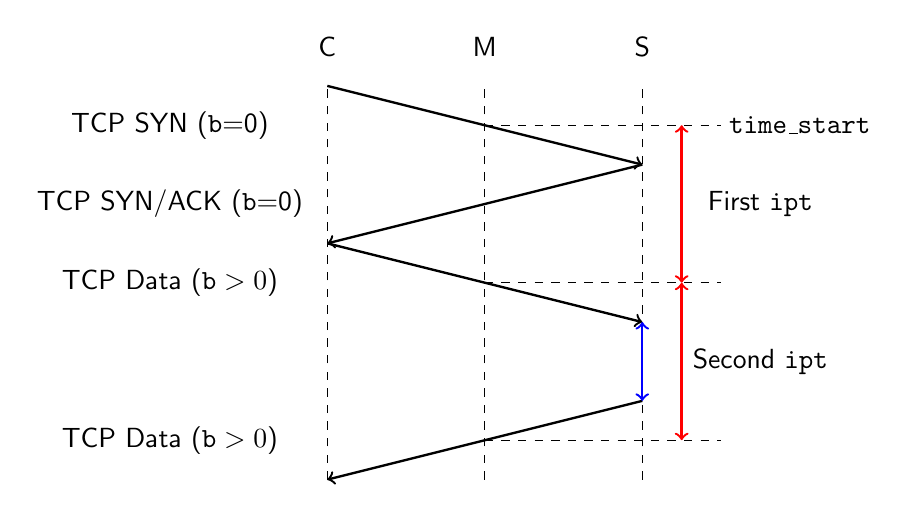
\begin{tikzpicture}
\node at (4,7.5) {S};
\node at (2,7.5) {M};
\node at (0,7.5) {C};
\draw[dashed] (0,2) -- (0,7);  
\draw[dashed] (4,2) -- (4,7);
\draw[dashed] (2,2) -- (2,7);  
\node at (-2,6.5) {TCP SYN (\texttt{b}=0)};
\draw[line width=.3mm,->] (0,7) -- (4,6);
\node at (-2,5.5) {TCP SYN/ACK (\texttt{b}=0)};
\draw[line width=.3mm,->] (4,6) -- (0,5);
\draw[dashed] (2,6.5) -- (5,6.5);
\node at (4.5,6) {};
\node at (6,6.5) {\texttt{time\_start}};
%\draw[dashed] (2,5.5) -- (5,5.5);
\node at (-2,4.5) {TCP Data ($\texttt{b}>0$)};
\node at (6,5.5) {};
\draw[line width=.3mm,<->,red] (4.5,6.5) -- (4.5,4.5);
\node at (5.5,5.5) {First \texttt{ipt}};
\draw[line width=.3mm,->] (0,5) -- (4,4);
\draw[line width=.3mm,->] (4,3) -- (0,2);
\draw[dashed] (2,4.5) -- (5,4.5);
\node at (6,4.5) {};
\draw[dashed] (2,2.5) -- (5,2.5);
\node at (-2,2.5) {TCP Data ($\texttt{b}>0$)};
\node at (6,2.5) {};
\draw[line width=.3mm,<->,red] (4.5,4.5) -- (4.5,2.5);
\draw[line width=.3mm,<->,blue] (4,4) -- (4,3);
\node at (5.5,3.5) {Second \texttt{ipt}};
\node at (4.5,3.5) {};
\end{tikzpicture}
\end{center}
\end{figure}



\section{JSON model for network data} 
JavaScript Object Notation (JSON~\cite{rfc7159}) excels at
representing complex data while at the same time being readable and
easily extensible.  That readability is essential making the data
useful; a person who does not understand the JSON format cannot write
queries or programs against it.  This note explains the conventions
that the \text{Joy} package uses to represent network data.  Its
goals are to faithfully represent as much data as possible, including
details such as the ordering of data elements and the capitalization
of text strings, and to have a schema that contains all of the
important data elements as explicitly named members.  This note
explains the conventions used to meet these goals.

\subsection{TLVs}
Many network protocols make use of a list or array of elements of
different types, with each element containing a type code that
indicates how it should be processed.  In the Type/Length/Value (TLV)
data representation, a message contains a list of elements, each of
which consists of a type code field containing an integer that
indicates how the element should be interpreted, a length field that
indicates the number of bytes in the element, and a value field that
contains the actual data.  The flexibility of the TLV representation
makes it well suited for network protocols, and its use is commonplace.
TCP options~\cite{rfc793,ianatcp} are an early example, though the acronym TLV
appeared later and was not used in the TCP specification;
we use that example to illustrate the \text{Joy} data-representation conventions.
Table~\ref{tcptable} summarizes the important TCP option types.
%In that
%example, the known data types include the MSS (an integer), WS (an
%integer), and TS (a pair of integers).

In a TLV scheme, some type codes are \textit{registered}, that is, the
format and interpretation of the value field for that type is well
defined and documented.  The data formats of known types are typically
defined in standards documents, and the type codes for IETF standards
are registered with the Internet Assigned Number Authority
(IANA)~\cite{iana}, as is the case for TCP Options~\cite{ianatcp}. Each
known type type has a (human readable) name, such as Maximum Segment
Size (MSS), Window Scale (WS), or Time Stamp (TS).  A type code that
is not registered may be \textit{unassigned} or \textit{reserved}.  An
unassigned type code is one that does not correspond to any registered
data format, and thus it is unknown how to interpret its value field.
Sometimes implementers define a new option but neglect to register it
with IANA, in which case IANA will typically reserve that type code,
so that it is moved out of the unassigned category.
%IANA known unauthorized use without proper IANA assignment
We say that a type code and its corresponding data format
are \textit{known} whenever they are registered, or whenever they are
reserved but with a known format.  

% The
%type code that appears in a message need not correspond to a known
%type; in IANA terms, a type code value may be \textit{reserved} for
%future use or private use.  In all of those cases, it is unknown how
%to interpret the value field.

\begin{table}
  \center
  \caption{The well-known TCP options.}
  \label{tcptable}
  \begin{tabular}{c|l|l|l} 
    Type &      Meaning         &  \text{Joy} Name    & \text{Joy} Value    \\ \hline
    0    & End of Option List   & -             & -             \\
    1    & No-Operation         & \texttt{noop} & \texttt{none}  \\
    2    & Maximum Segment Size & \texttt{mss}  & number        \\
    3    & Window Scale         & \texttt{ws}   & number        \\
    4    & SACK Permitted       & \texttt{sackp}& \texttt{none} \\
    5    & SACK                 & \texttt{sack} & hex string    \\
%    6    & Echo (obsoleted by option 8)       & & ?             \\
%    7    & Echo Reply (obsoleted by option 8) & & ?             \\
    8    & Timestamps           & \texttt{ts}   & object
  \end{tabular}
\end{table}

\subsection{Conventions}
When representing a list of TLV elements in JSON, \text{Joy} uses the
following conventions.  The list is represented in JSON as an array of
objects, ordered as the elements appear in the message, and each
object as follows:
\begin{itemize}
%\item a member with the name \texttt{type}, whose value is the type number
%  from the TLV element,
%\item a member with the name \texttt{length}, whose value is the length
%  number from the TLV element,
\item if the type code is known, the object contains a member whose JSON name is the
  human-readable name associated with the type code, such as \texttt{mss} for
  the TCP MSS option, and whose JSON value can be a string, array, \texttt{null}, \texttt{false}, \texttt{true}, or
  object, as is appropriate to represent the value of that particular
  TLV element,
\item if the type is unknown, the object contains a
  member with the JSON name \texttt{type} whose JSON value
  is a numeric representation of the type code, and a member
  whose JSON name is \texttt{data} whose value is a
  hexadecimal representation of the value from the TLV element.
%\item if the type is unknown, the object contains a
%  member whose name is the string representation of the type, such as
%  \texttt{79} for the TCP reserved type 79, and whose value is a
%  hexadecimal representation of the value from the TLV element.
\end{itemize}
Additionally, all member names contain only non-whitespace characters,
so that those names need not be quoted in JSON tools.
%The convention to omit whitespace characters from JSON strings allows
%to avoid escaping space characters in JSON tools.

With these conventions, there is no need for a user or a program to
memorize or understand the type codes that have been registered.
Known types are represented as recognizable member names in the JSON
schema, and unknown types are represented by \texttt{type} and
\texttt{data} fields.  Known types can easily be accessed, while the
schema for unknown types is regular.  
%With this representation, the JSON schema contains the human-readable
%names for all of the known data types.
Importantly, the conventions ensure that the JSON schema contains the
information needed to understand the JSON data.  The important
information is present in JSON member names, instead of residing in a
JSON value.
For instance, the TCP options are represented as

\begin{minipage}{\textwidth}
\begin{minted}{javascript} 
      {
         "opts": [
            {
               "mss": 1460
            }, 
            {
               "sackp": null 
            }, 
            {
               "ts": {
                  "val": 4332608, 
                  "ecr": 0
                }
            }, 
            {
               "noop": null
            }, 
            {
               "ws": 7
            },
            {
               "type": 79,
               "data": "abadcafe"
            }
         ]
      }
\end{minted} 
\end{minipage}

The JSON schema for TCP options is:

\begin{minipage}{\textwidth}
\begin{minted}{javascript}
{
  "required": [
    "opts"
  ], 
  "type": "object", 
  "properties": {
    "opts": {
      "items": {
        "type": "object", 
        "properties": {
          "sackp": {
            "type": "null"
          }, 
          "mss": {
            "type": "integer"
          }, 
          "ts": {
            "required": [
              "ecr", 
              "val"
            ], 
            "type": "object", 
            "properties": {
              "ecr": {
                "type": "integer"
              }, 
              "val": {
                "type": "integer"
              }
            }
          }, 
          "noop": {
            "type": "null"
          }, 
          "ws": {
            "type": "integer"
          }, 
          "data": {
            "type": "string"
          }
        }
      }, 
      "type": "array"
    }
  }
}
\end{minted}
\end{minipage}



\subsubsection{What does it look like when these conventions aren't followed?}
In contrast, the  method of having the JSON schema for a TLV element
contain members with the JSON names type, length, and data
makes that schema devoid of the detailed information of how to
interpret the data values, and forces the JSON user to use the
\texttt{type} member as an index or search value for the
\texttt{data}, and forces the JSON tools to interpret the
\texttt{data} member in a type-specific way.  This method
results in a schema of
\begin{minted}{javascript}
   "opts": { 
     "properties": { 
        "type": "number", 
        "length": "number", 
        "data": "string" 
      }
   }
\end{minted}
which gives no information about what type numbers might appear in the
JSON.  Furthermore, it is awkward to search with this schema, since
searching for the \texttt{data} JSON values corresponding to
particular \texttt{type} JSON value requires that the search tool
report one value based on a search query corresponding to a different
value.




\bibliographystyle{plain} 
\bibliography{ieeesecpriv,rfc,mcgrew,johnq,pevnak}


\end{document}  

\begin{document}



\end{document}